\documentclass[11pt]{article}
\usepackage[textwidth=18.0cm, textheight=23.0cm, top=2.0cm]{geometry}
\usepackage{pst-all}
\usepackage{amssymb}
\usepackage{tikz}
\usepackage{underscore}\begin{document}
\pagestyle{empty}


ClassName: \underline{\textbf{Class_03.2bp-21}}
\par
BinSize: \underline{\textbf{40 × 40}}
\par
ReduceSize: \underline{\textbf{40 × 40}}
\par
TypeNum: \underline{\textbf{58}}
\par
Num: \underline{\textbf{60}}
\par
OutS: \underline{\textbf{20800}}
\par
InS: \underline{\textbf{18220}}
\par
Rate: \underline{\textbf{0.876}}
\par
UB: \underline{\textbf{13}}
\par
LB0: \underline{\textbf{13}}
\par
LB: \underline{\textbf{13}}
\par
LBWithCut: \underline{\textbf{13}}
\par
NodeCut: \underline{\textbf{0}}
\par
ExtendedNodeCnt: \underline{\textbf{1}}
\par
GenNodeCnt: \underline{\textbf{1}}
\par
PrimalNode: \underline{\textbf{0}}
\par
ColumnCount: \underline{\textbf{13}}
\par
TotalCutCount: \underline{\textbf{0}}
\par
RootCutCount: \underline{\textbf{0}}
\par
LPSolverCnt: \underline{\textbf{1}}
\par
PricingSolverCnt: \underline{\textbf{0}}
\par
BranchAndBoundNum: \underline{\textbf{1}}
\par
isOpt: \underline{\textbf{true}}
\par
TimeOnInitSolution: \underline{\textbf{600.000 s}}
\par
TimeOnPrimal: \underline{\textbf{0.000 s}}
\par
TimeOnPricing: \underline{\textbf{0.000 s}}
\par
TimeOnRmp: \underline{\textbf{0.078 s}}
\par
TotalTime: \underline{\textbf{600.328 s}}
\par
\newpage


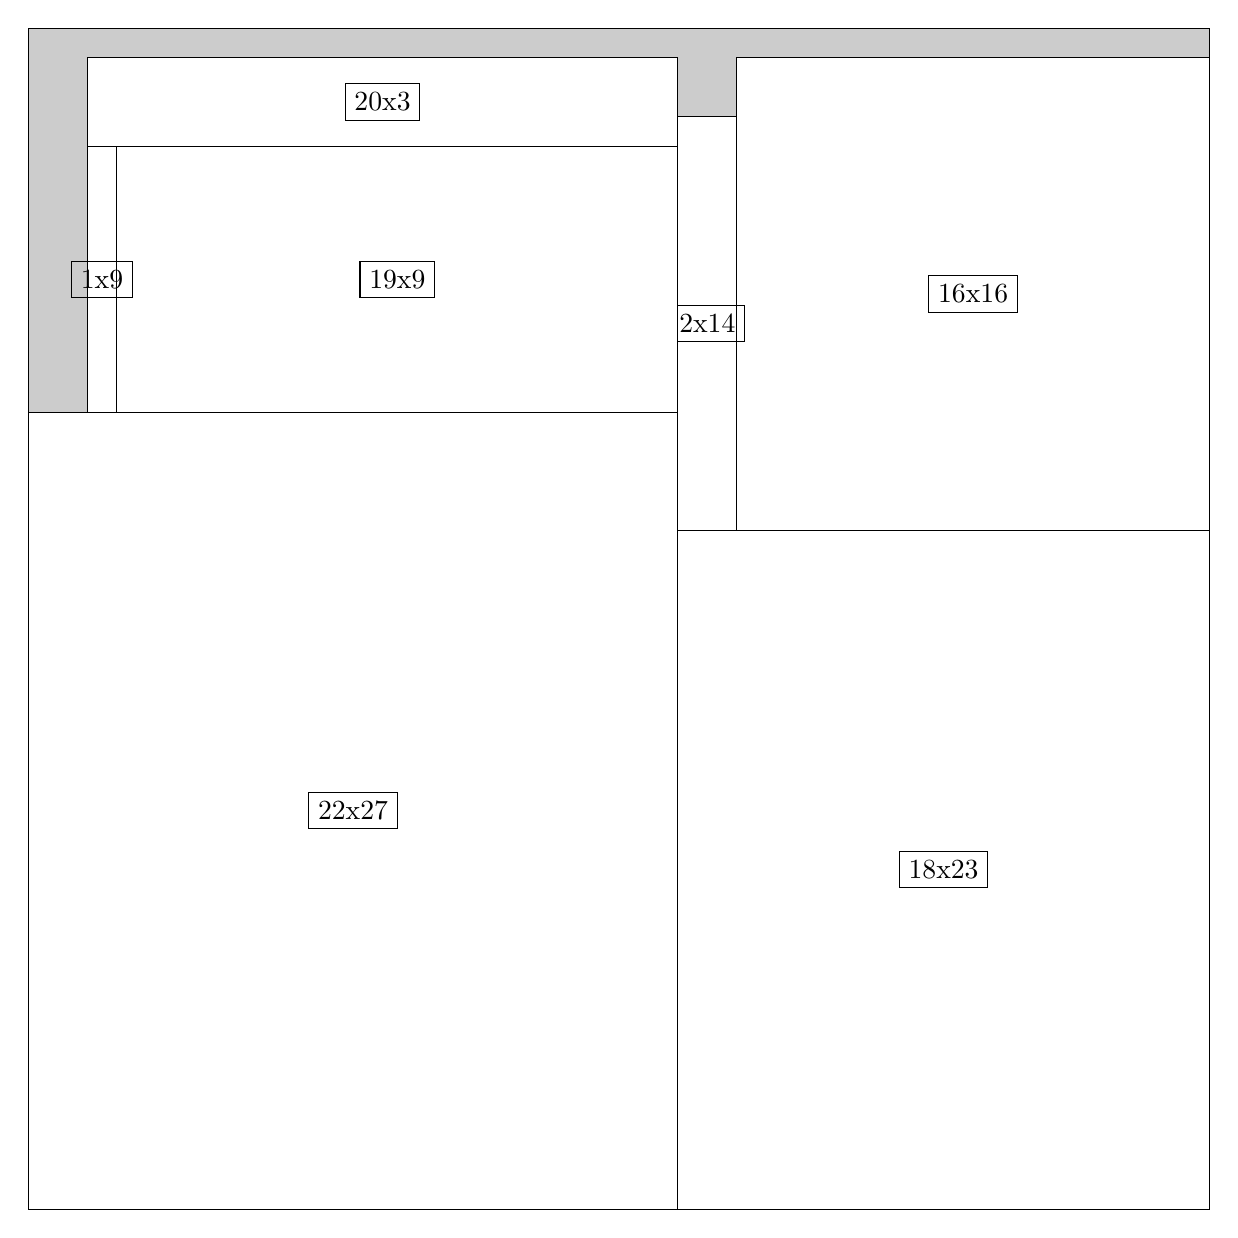
\begin{tikzpicture}[shorten >=1pt,scale=1.0,every node/.style={scale=1.0},->]
\tikzstyle{vertex}=[circle,fill=black!25,minimum size=14pt,inner sep=0pt]
\filldraw[fill=gray!40!white, draw=black] (0,0) rectangle (15.0,15.0);
\foreach \name/\x/\y/\w/\h in {18x23/8.25/0.0/6.75/8.625,16x16/9.0/8.625/6.0/6.0,2x14/8.25/8.625/0.75/5.25,22x27/0.0/0.0/8.25/10.125,19x9/1.125/10.125/7.125/3.375,1x9/0.75/10.125/0.375/3.375,20x3/0.75/13.5/7.5/1.125}
\filldraw[fill=white!40!white, draw=black] (\x,\y) rectangle node[draw] (\name) {\name} ++(\w,\h);
\end{tikzpicture}


w =18 , h =23 , x =22 , y =0 , v =414
\par
w =16 , h =16 , x =24 , y =23 , v =256
\par
w =2 , h =14 , x =22 , y =23 , v =28
\par
w =22 , h =27 , x =0 , y =0 , v =594
\par
w =19 , h =9 , x =3 , y =27 , v =171
\par
w =1 , h =9 , x =2 , y =27 , v =9
\par
w =20 , h =3 , x =2 , y =36 , v =60
\par
\newpage


\begin{tikzpicture}[shorten >=1pt,scale=1.0,every node/.style={scale=1.0},->]
\tikzstyle{vertex}=[circle,fill=black!25,minimum size=14pt,inner sep=0pt]
\filldraw[fill=gray!40!white, draw=black] (0,0) rectangle (15.0,15.0);
\foreach \name/\x/\y/\w/\h in {29x22/4.125/0.0/10.875/8.25,11x22/0.0/0.0/4.125/8.25,34x18/2.25/8.25/12.75/6.75,5x16/0.375/8.25/1.875/6.0,1x15/0.0/8.25/0.375/5.625}
\filldraw[fill=white!40!white, draw=black] (\x,\y) rectangle node[draw] (\name) {\name} ++(\w,\h);
\end{tikzpicture}


w =29 , h =22 , x =11 , y =0 , v =638
\par
w =11 , h =22 , x =0 , y =0 , v =242
\par
w =34 , h =18 , x =6 , y =22 , v =612
\par
w =5 , h =16 , x =1 , y =22 , v =80
\par
w =1 , h =15 , x =0 , y =22 , v =15
\par
\newpage


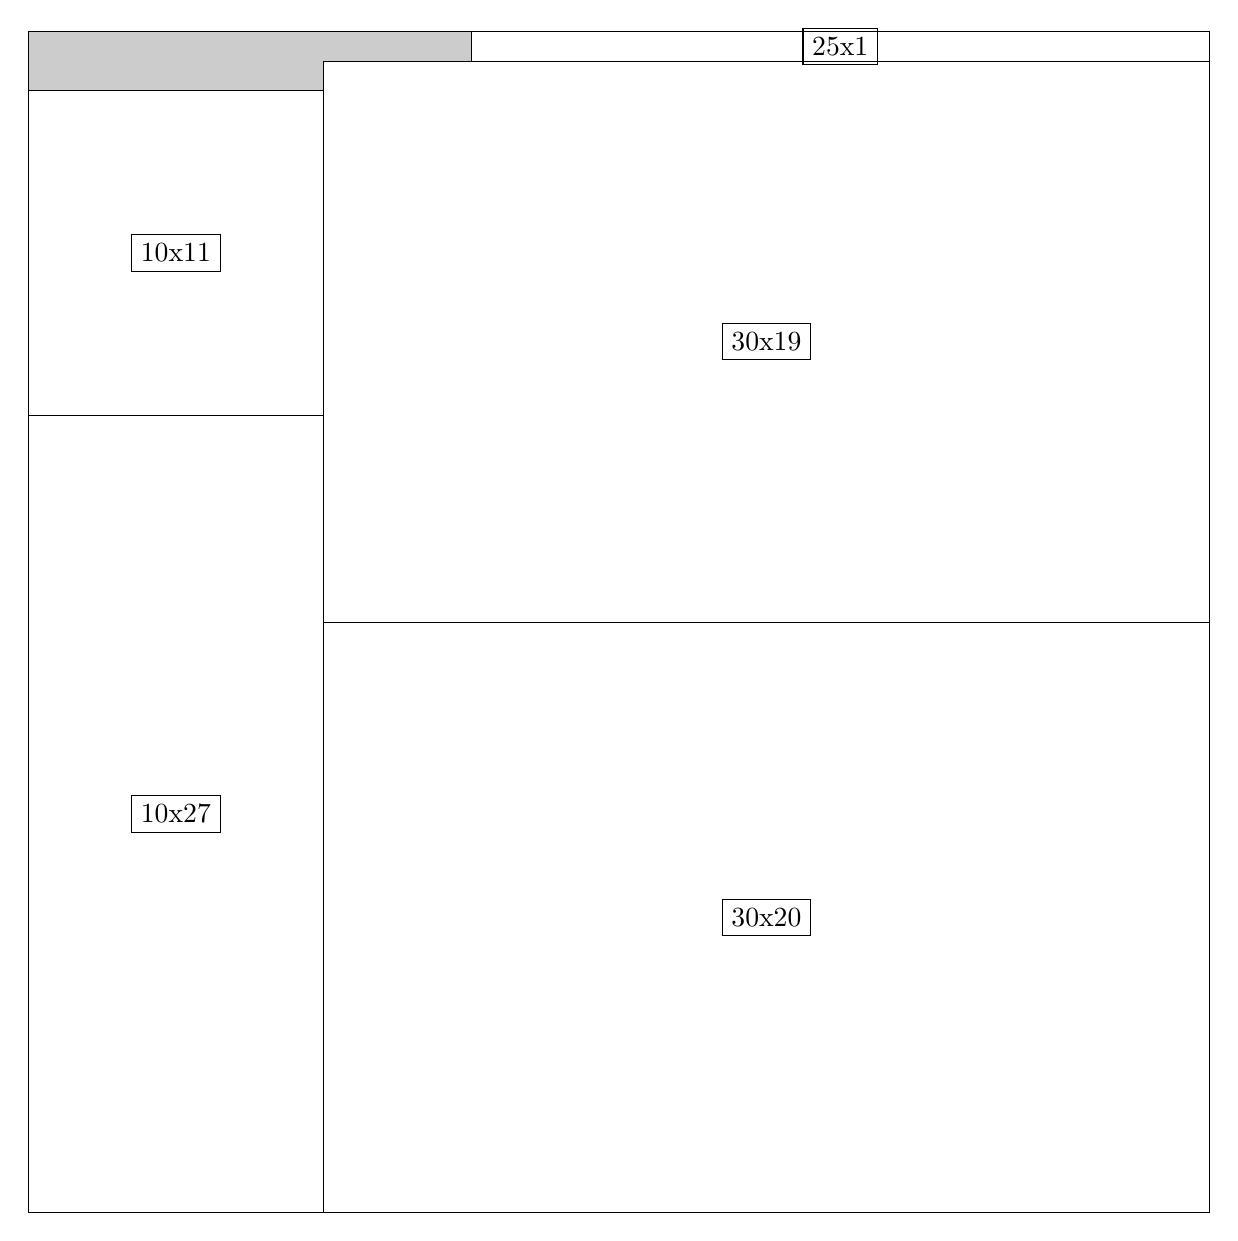
\begin{tikzpicture}[shorten >=1pt,scale=1.0,every node/.style={scale=1.0},->]
\tikzstyle{vertex}=[circle,fill=black!25,minimum size=14pt,inner sep=0pt]
\filldraw[fill=gray!40!white, draw=black] (0,0) rectangle (15.0,15.0);
\foreach \name/\x/\y/\w/\h in {30x20/3.75/0.0/11.25/7.5,30x19/3.75/7.5/11.25/7.125,25x1/5.625/14.625/9.375/0.375,10x27/0.0/0.0/3.75/10.125,10x11/0.0/10.125/3.75/4.125}
\filldraw[fill=white!40!white, draw=black] (\x,\y) rectangle node[draw] (\name) {\name} ++(\w,\h);
\end{tikzpicture}


w =30 , h =20 , x =10 , y =0 , v =600
\par
w =30 , h =19 , x =10 , y =20 , v =570
\par
w =25 , h =1 , x =15 , y =39 , v =25
\par
w =10 , h =27 , x =0 , y =0 , v =270
\par
w =10 , h =11 , x =0 , y =27 , v =110
\par
\newpage


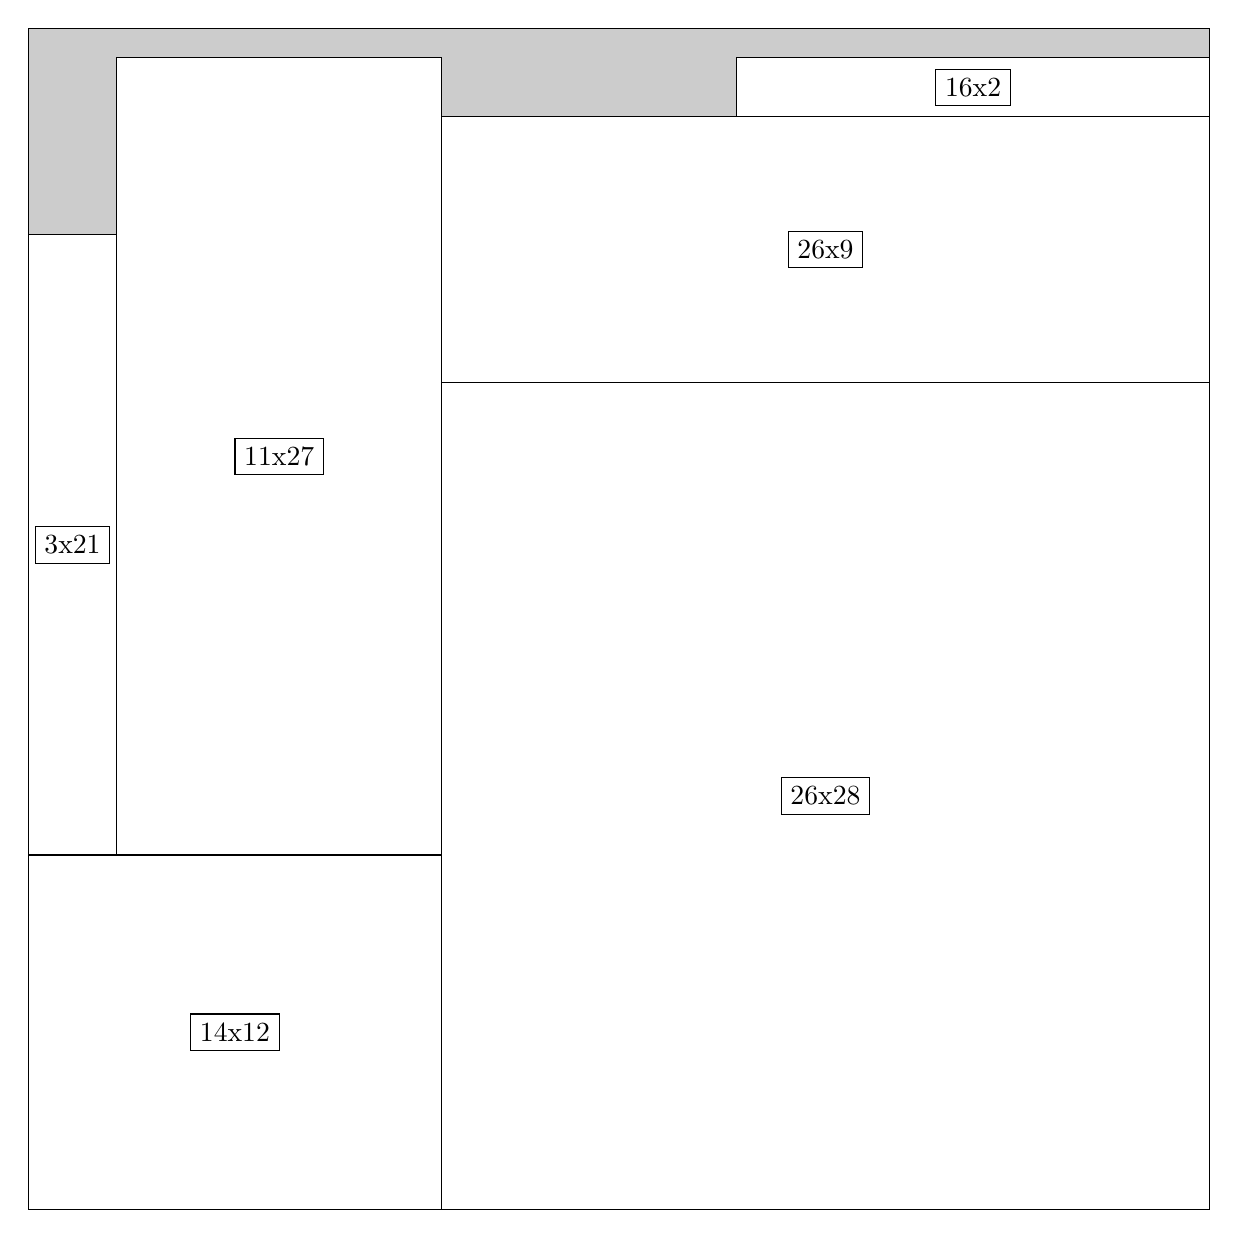
\begin{tikzpicture}[shorten >=1pt,scale=1.0,every node/.style={scale=1.0},->]
\tikzstyle{vertex}=[circle,fill=black!25,minimum size=14pt,inner sep=0pt]
\filldraw[fill=gray!40!white, draw=black] (0,0) rectangle (15.0,15.0);
\foreach \name/\x/\y/\w/\h in {26x28/5.25/0.0/9.75/10.5,26x9/5.25/10.5/9.75/3.375,16x2/9.0/13.875/6.0/0.75,14x12/0.0/0.0/5.25/4.5,11x27/1.125/4.5/4.125/10.125,3x21/0.0/4.5/1.125/7.875}
\filldraw[fill=white!40!white, draw=black] (\x,\y) rectangle node[draw] (\name) {\name} ++(\w,\h);
\end{tikzpicture}


w =26 , h =28 , x =14 , y =0 , v =728
\par
w =26 , h =9 , x =14 , y =28 , v =234
\par
w =16 , h =2 , x =24 , y =37 , v =32
\par
w =14 , h =12 , x =0 , y =0 , v =168
\par
w =11 , h =27 , x =3 , y =12 , v =297
\par
w =3 , h =21 , x =0 , y =12 , v =63
\par
\newpage


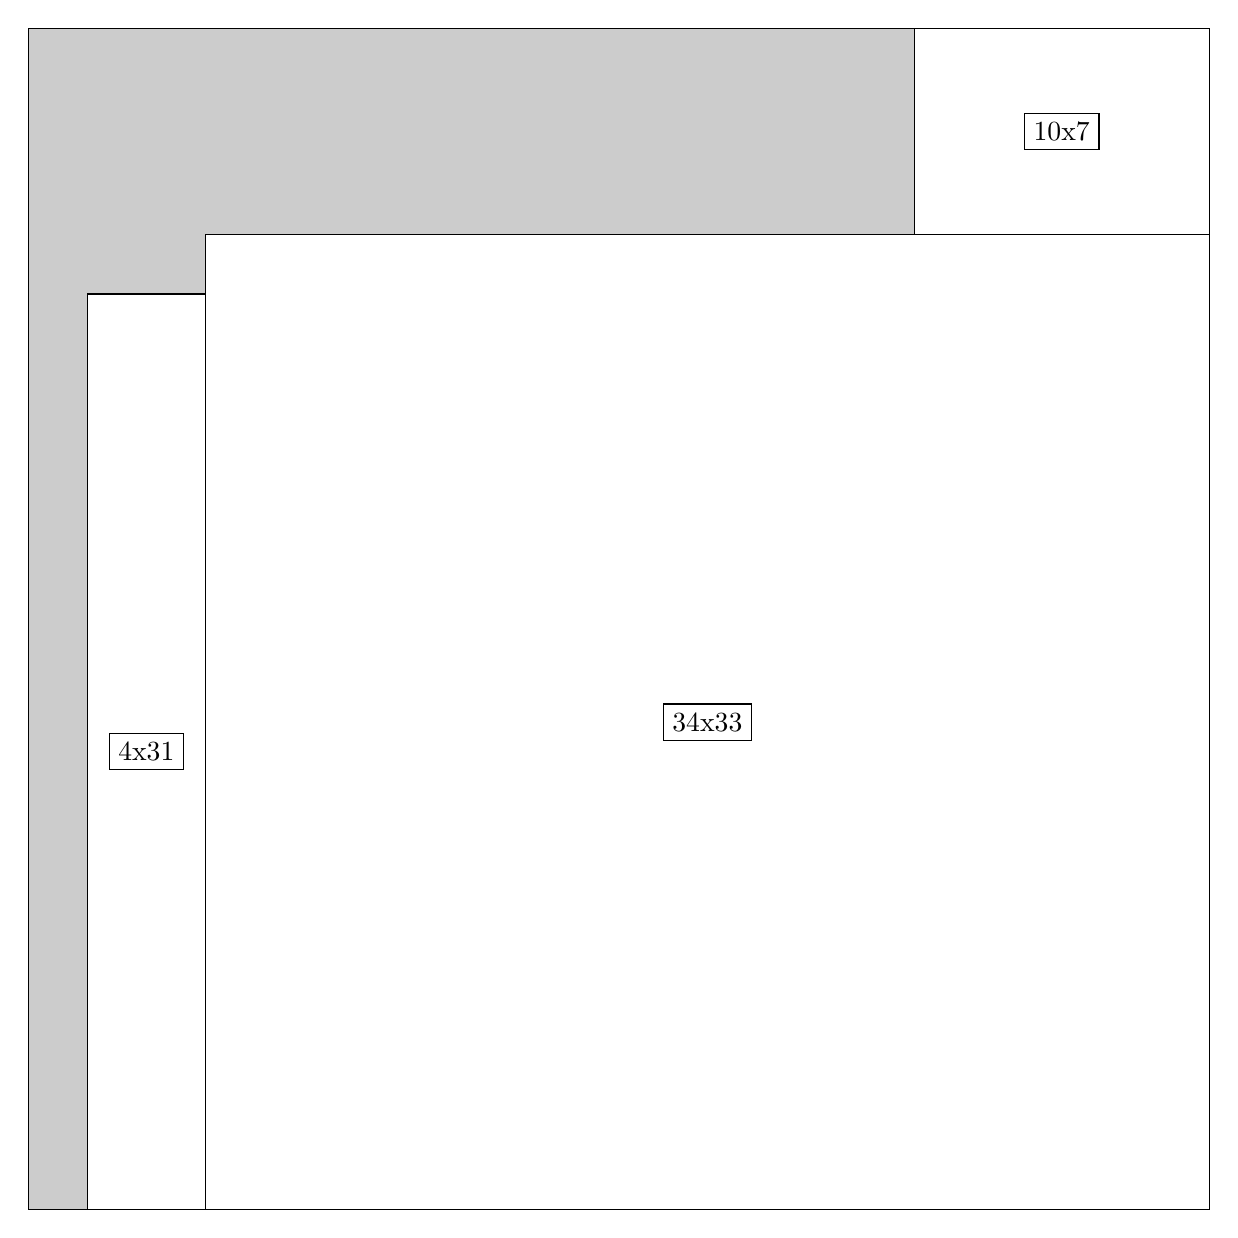
\begin{tikzpicture}[shorten >=1pt,scale=1.0,every node/.style={scale=1.0},->]
\tikzstyle{vertex}=[circle,fill=black!25,minimum size=14pt,inner sep=0pt]
\filldraw[fill=gray!40!white, draw=black] (0,0) rectangle (15.0,15.0);
\foreach \name/\x/\y/\w/\h in {34x33/2.25/0.0/12.75/12.375,10x7/11.25/12.375/3.75/2.625,4x31/0.75/0.0/1.5/11.625}
\filldraw[fill=white!40!white, draw=black] (\x,\y) rectangle node[draw] (\name) {\name} ++(\w,\h);
\end{tikzpicture}


w =34 , h =33 , x =6 , y =0 , v =1122
\par
w =10 , h =7 , x =30 , y =33 , v =70
\par
w =4 , h =31 , x =2 , y =0 , v =124
\par
\newpage


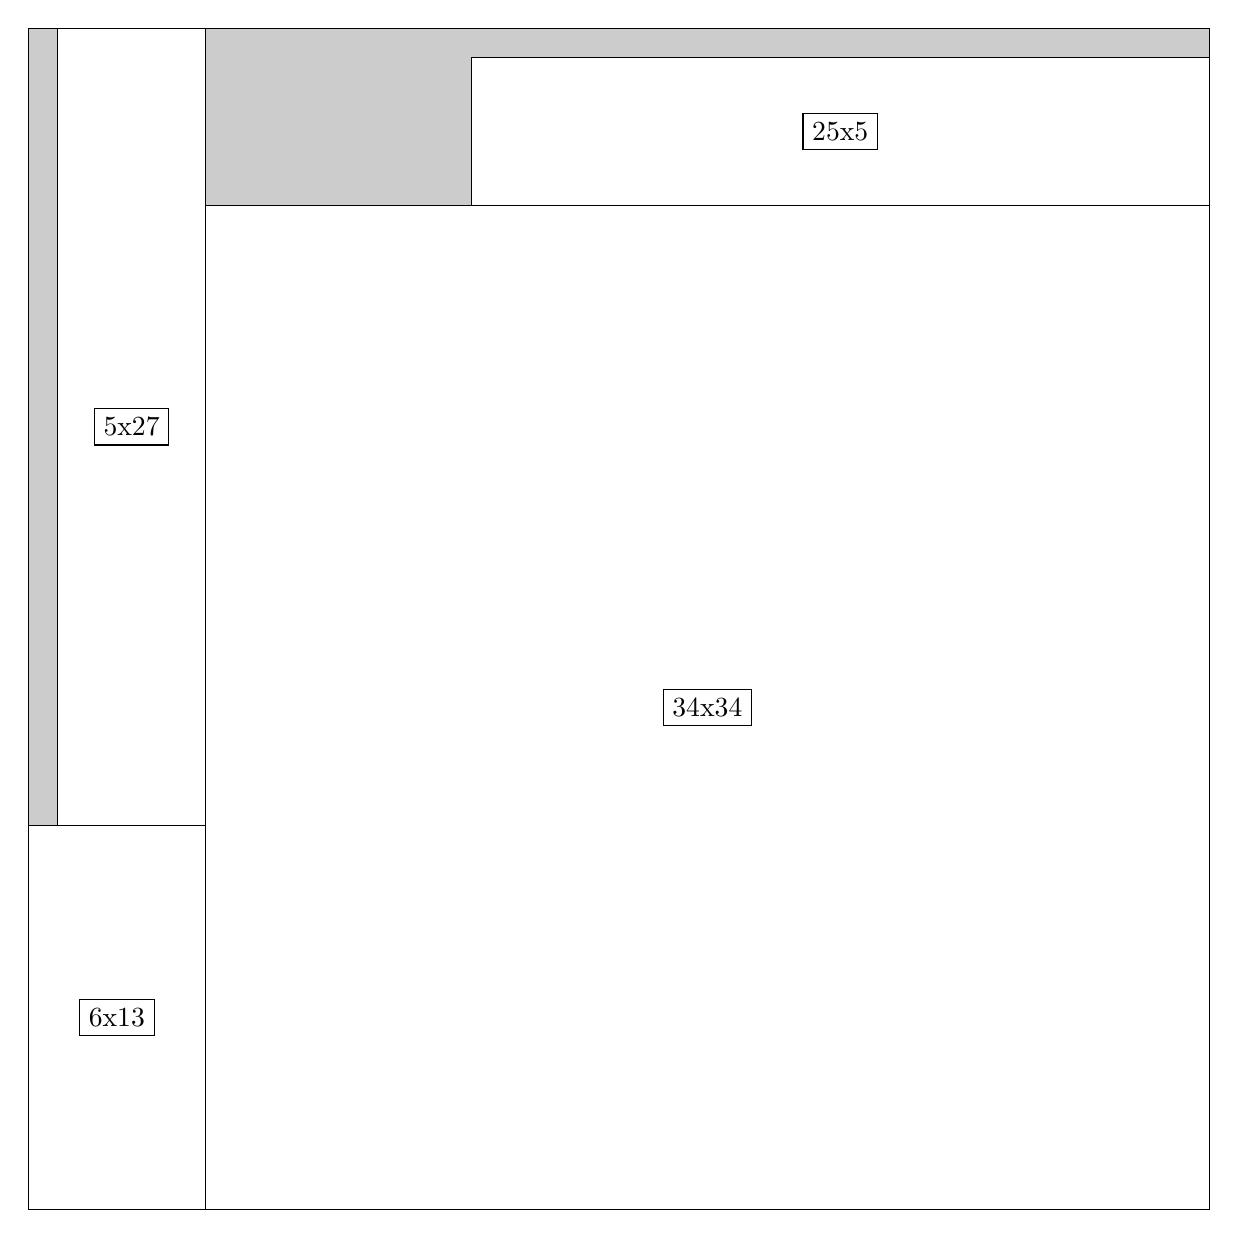
\begin{tikzpicture}[shorten >=1pt,scale=1.0,every node/.style={scale=1.0},->]
\tikzstyle{vertex}=[circle,fill=black!25,minimum size=14pt,inner sep=0pt]
\filldraw[fill=gray!40!white, draw=black] (0,0) rectangle (15.0,15.0);
\foreach \name/\x/\y/\w/\h in {34x34/2.25/0.0/12.75/12.75,25x5/5.625/12.75/9.375/1.875,6x13/0.0/0.0/2.25/4.875,5x27/0.375/4.875/1.875/10.125}
\filldraw[fill=white!40!white, draw=black] (\x,\y) rectangle node[draw] (\name) {\name} ++(\w,\h);
\end{tikzpicture}


w =34 , h =34 , x =6 , y =0 , v =1156
\par
w =25 , h =5 , x =15 , y =34 , v =125
\par
w =6 , h =13 , x =0 , y =0 , v =78
\par
w =5 , h =27 , x =1 , y =13 , v =135
\par
\newpage


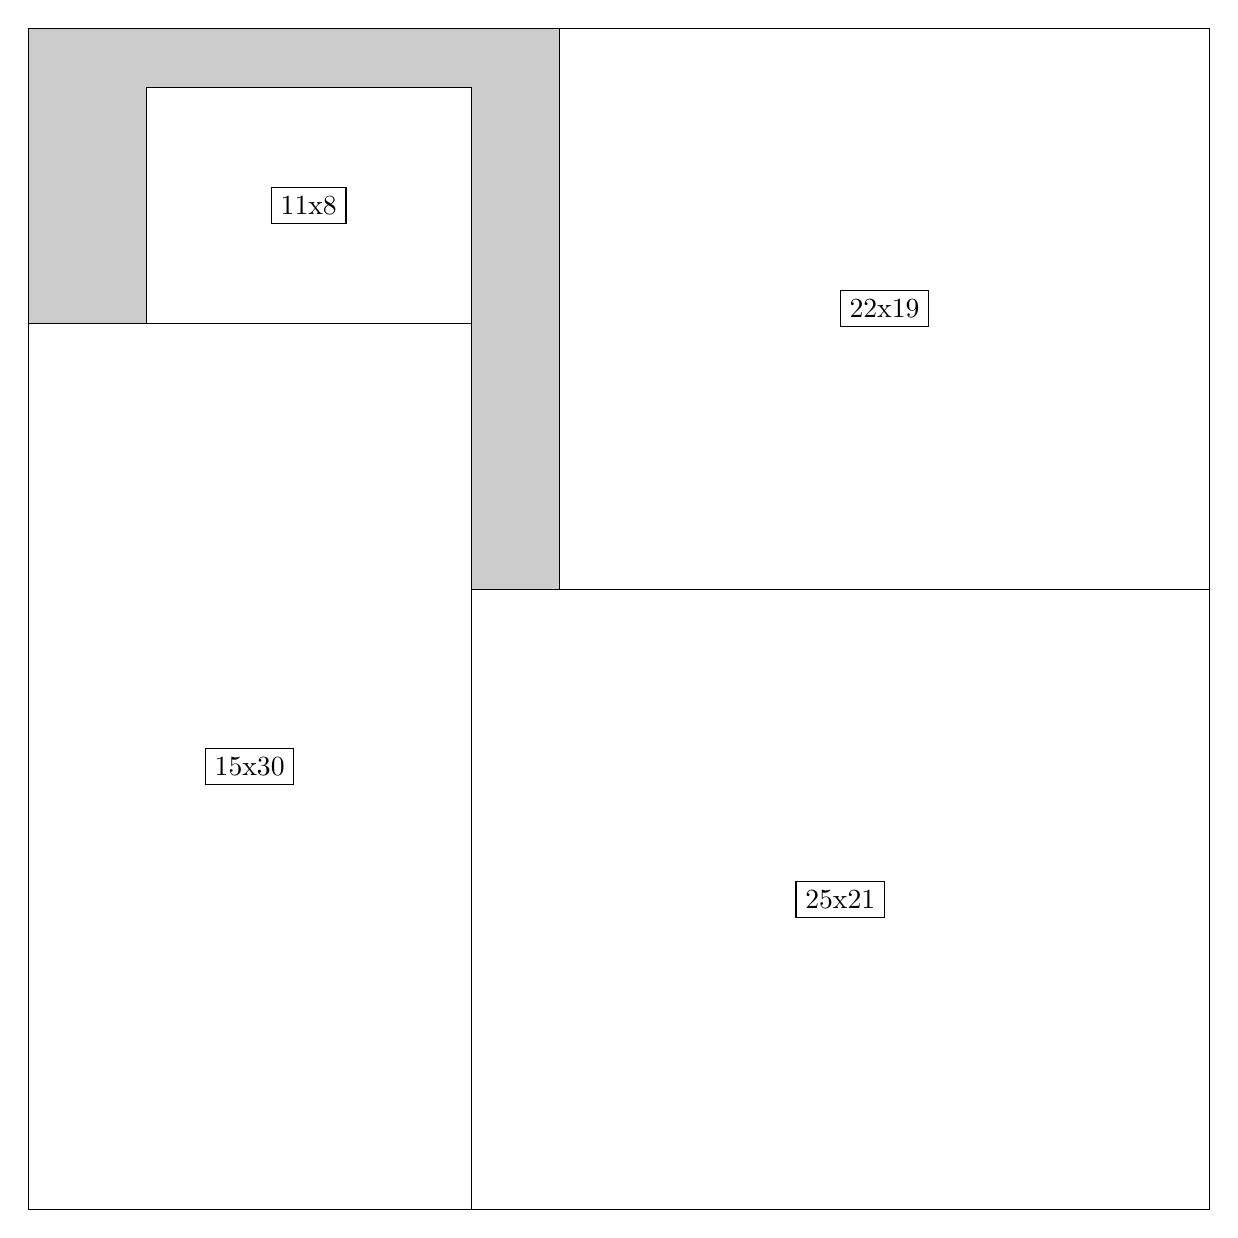
\begin{tikzpicture}[shorten >=1pt,scale=1.0,every node/.style={scale=1.0},->]
\tikzstyle{vertex}=[circle,fill=black!25,minimum size=14pt,inner sep=0pt]
\filldraw[fill=gray!40!white, draw=black] (0,0) rectangle (15.0,15.0);
\foreach \name/\x/\y/\w/\h in {25x21/5.625/0.0/9.375/7.875,22x19/6.75/7.875/8.25/7.125,15x30/0.0/0.0/5.625/11.25,11x8/1.5/11.25/4.125/3.0}
\filldraw[fill=white!40!white, draw=black] (\x,\y) rectangle node[draw] (\name) {\name} ++(\w,\h);
\end{tikzpicture}


w =25 , h =21 , x =15 , y =0 , v =525
\par
w =22 , h =19 , x =18 , y =21 , v =418
\par
w =15 , h =30 , x =0 , y =0 , v =450
\par
w =11 , h =8 , x =4 , y =30 , v =88
\par
\newpage


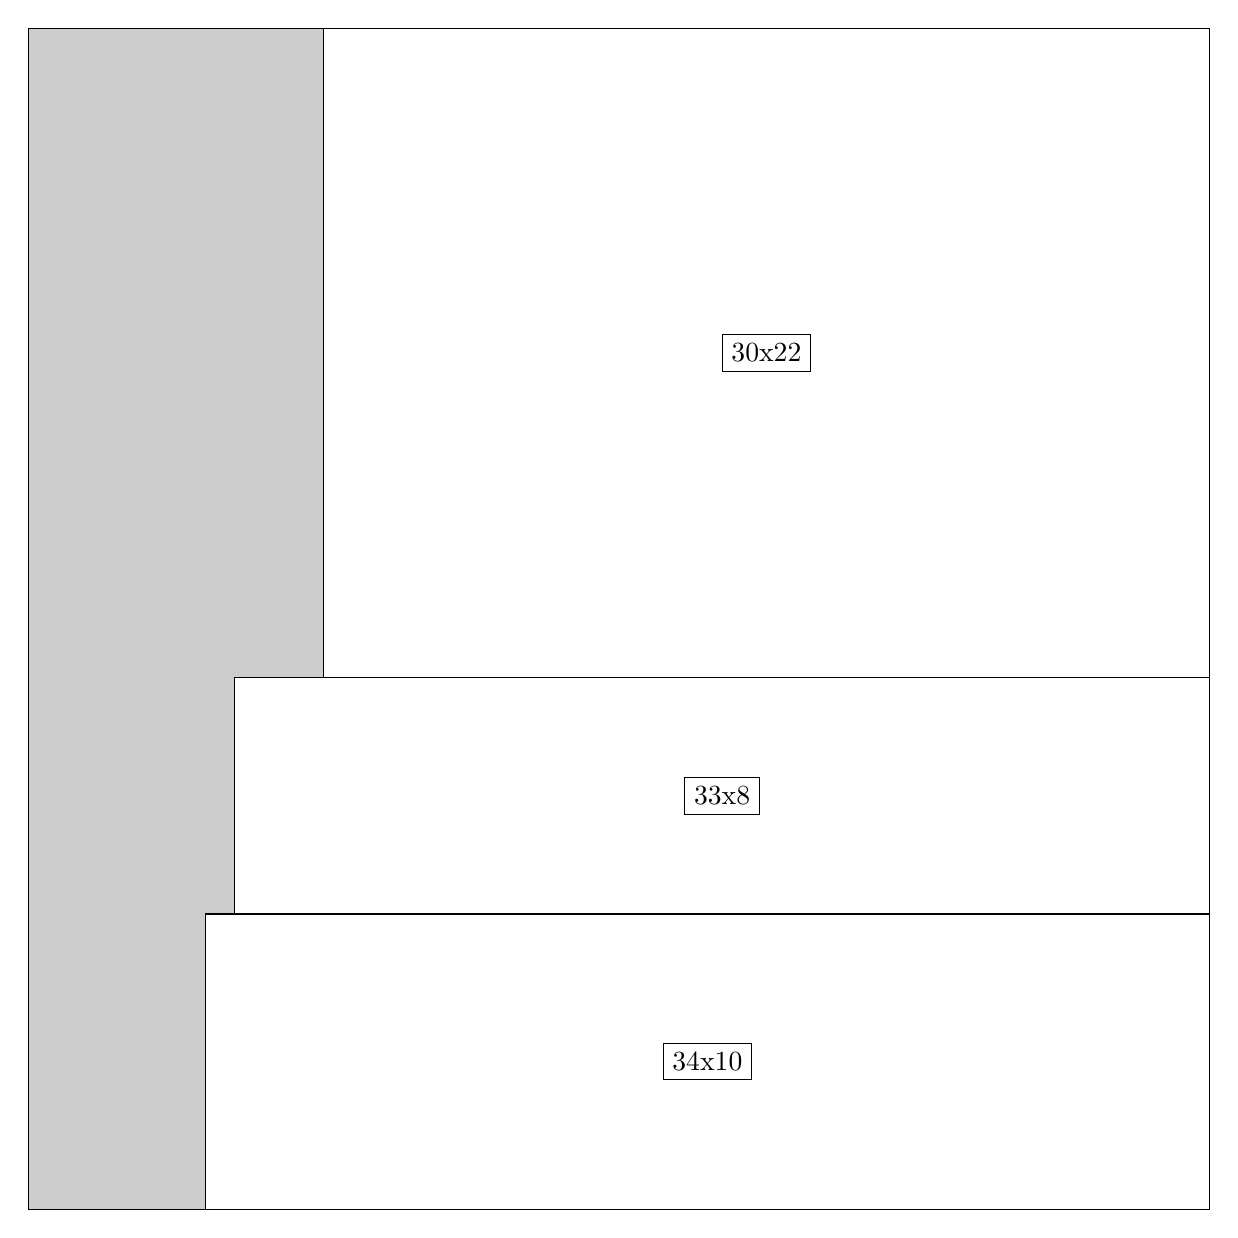
\begin{tikzpicture}[shorten >=1pt,scale=1.0,every node/.style={scale=1.0},->]
\tikzstyle{vertex}=[circle,fill=black!25,minimum size=14pt,inner sep=0pt]
\filldraw[fill=gray!40!white, draw=black] (0,0) rectangle (15.0,15.0);
\foreach \name/\x/\y/\w/\h in {34x10/2.25/0.0/12.75/3.75,33x8/2.625/3.75/12.375/3.0,30x22/3.75/6.75/11.25/8.25}
\filldraw[fill=white!40!white, draw=black] (\x,\y) rectangle node[draw] (\name) {\name} ++(\w,\h);
\end{tikzpicture}


w =34 , h =10 , x =6 , y =0 , v =340
\par
w =33 , h =8 , x =7 , y =10 , v =264
\par
w =30 , h =22 , x =10 , y =18 , v =660
\par
\newpage


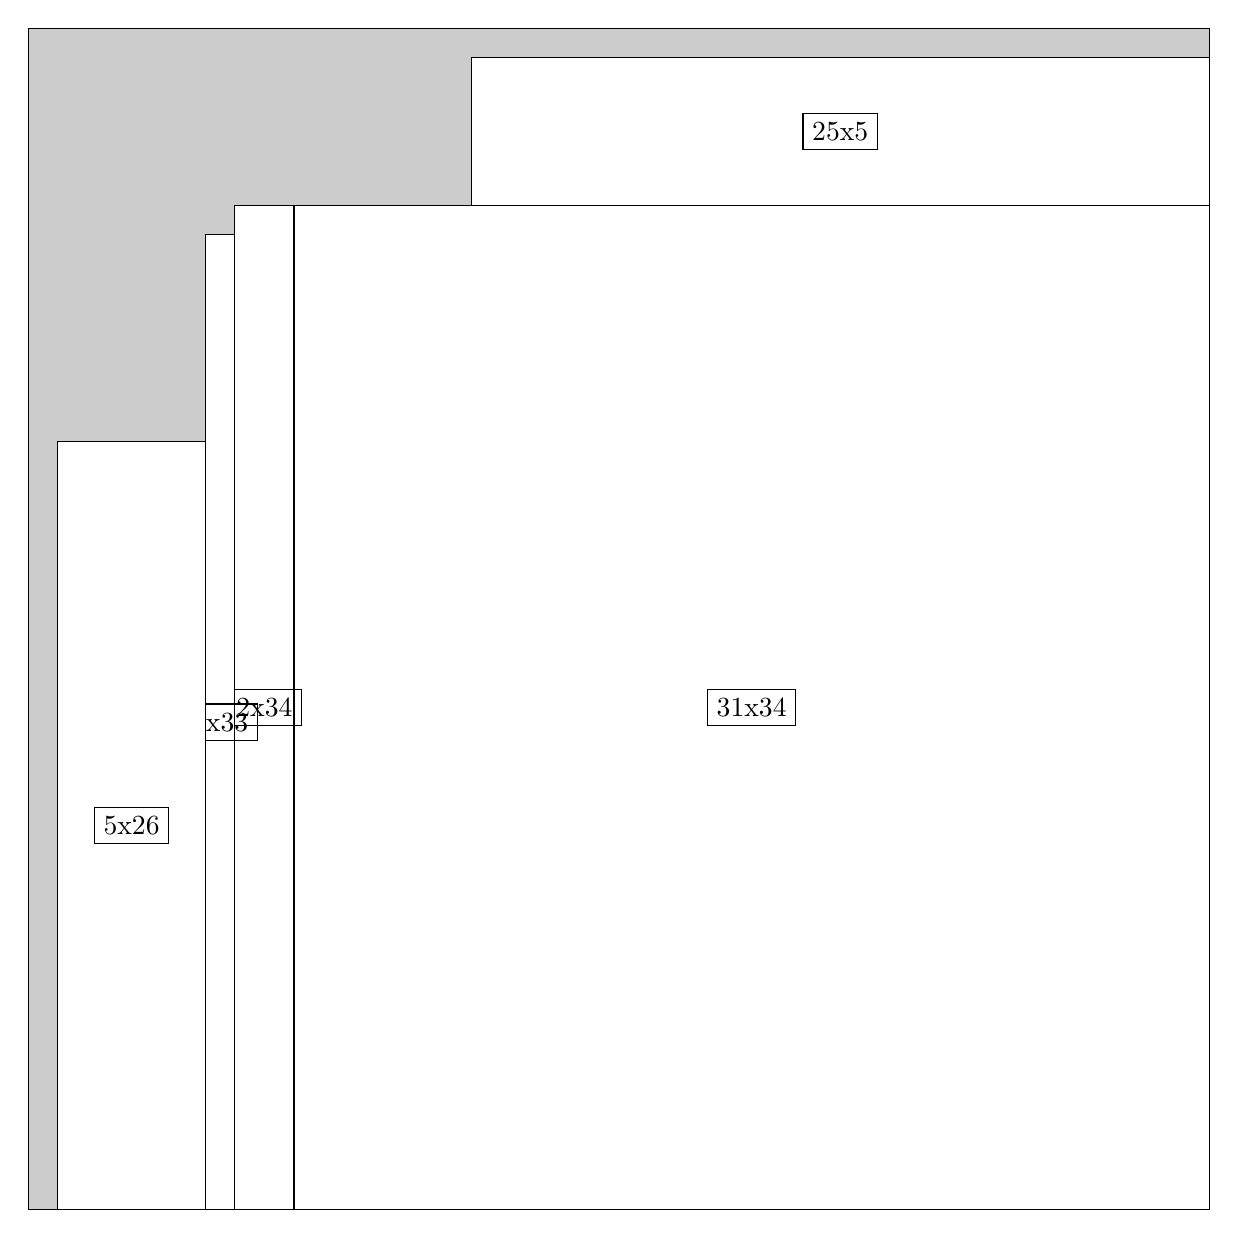
\begin{tikzpicture}[shorten >=1pt,scale=1.0,every node/.style={scale=1.0},->]
\tikzstyle{vertex}=[circle,fill=black!25,minimum size=14pt,inner sep=0pt]
\filldraw[fill=gray!40!white, draw=black] (0,0) rectangle (15.0,15.0);
\foreach \name/\x/\y/\w/\h in {31x34/3.375/0.0/11.625/12.75,2x34/2.625/0.0/0.75/12.75,1x33/2.25/0.0/0.375/12.375,5x26/0.375/0.0/1.875/9.75,25x5/5.625/12.75/9.375/1.875}
\filldraw[fill=white!40!white, draw=black] (\x,\y) rectangle node[draw] (\name) {\name} ++(\w,\h);
\end{tikzpicture}


w =31 , h =34 , x =9 , y =0 , v =1054
\par
w =2 , h =34 , x =7 , y =0 , v =68
\par
w =1 , h =33 , x =6 , y =0 , v =33
\par
w =5 , h =26 , x =1 , y =0 , v =130
\par
w =25 , h =5 , x =15 , y =34 , v =125
\par
\newpage


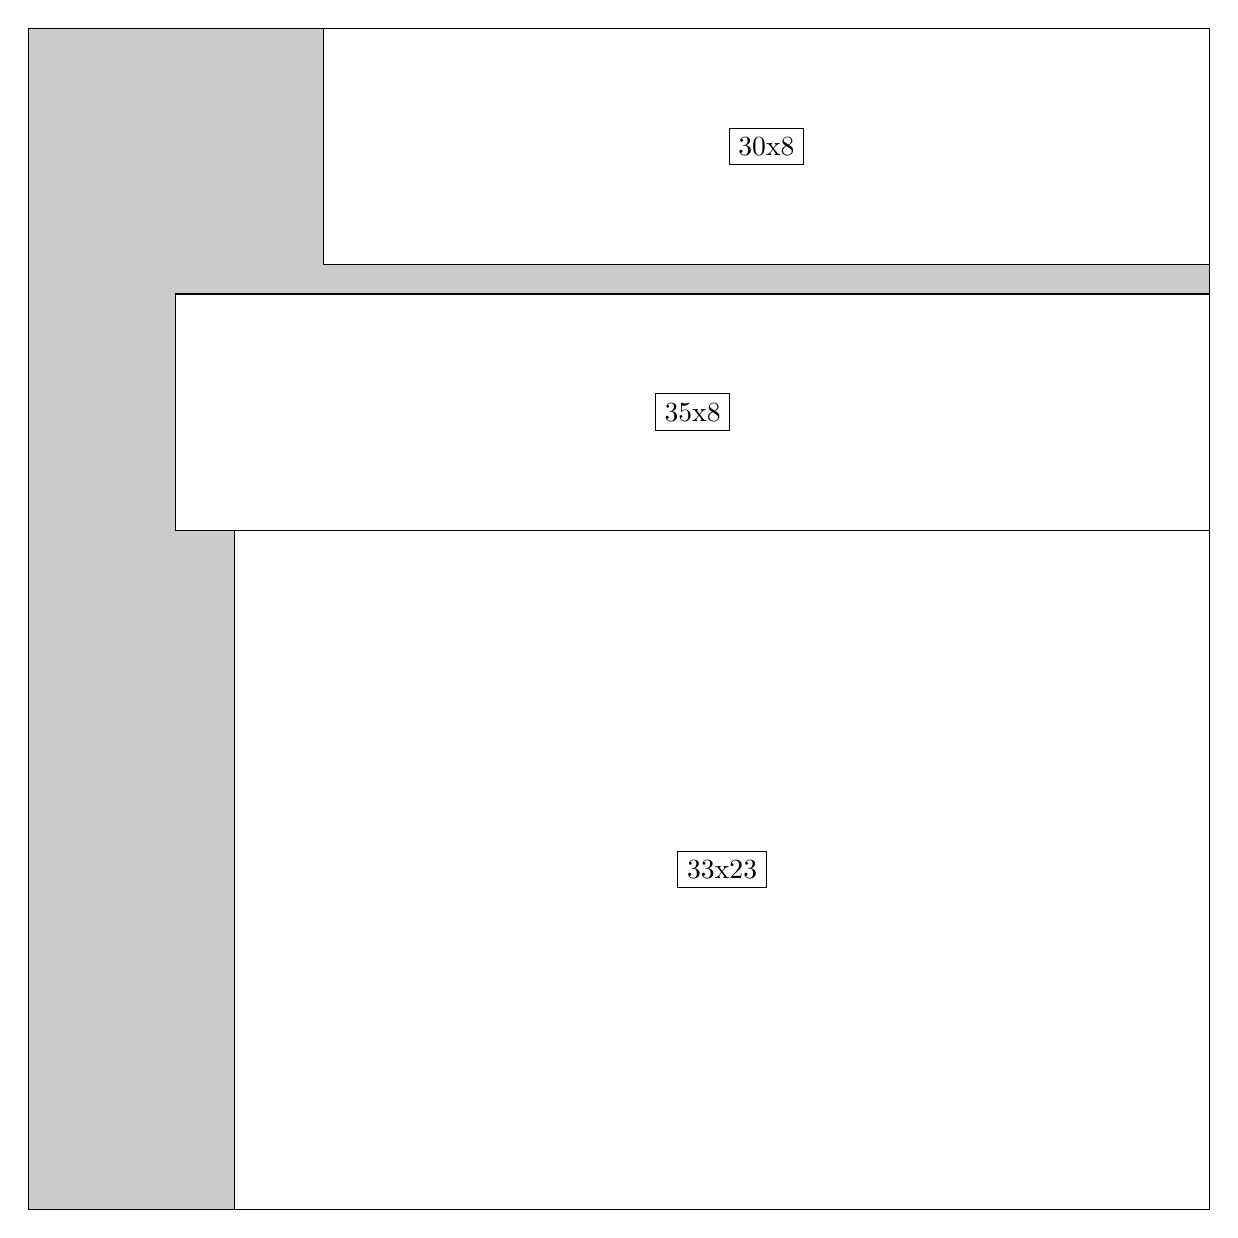
\begin{tikzpicture}[shorten >=1pt,scale=1.0,every node/.style={scale=1.0},->]
\tikzstyle{vertex}=[circle,fill=black!25,minimum size=14pt,inner sep=0pt]
\filldraw[fill=gray!40!white, draw=black] (0,0) rectangle (15.0,15.0);
\foreach \name/\x/\y/\w/\h in {33x23/2.625/0.0/12.375/8.625,35x8/1.875/8.625/13.125/3.0,30x8/3.75/12.0/11.25/3.0}
\filldraw[fill=white!40!white, draw=black] (\x,\y) rectangle node[draw] (\name) {\name} ++(\w,\h);
\end{tikzpicture}


w =33 , h =23 , x =7 , y =0 , v =759
\par
w =35 , h =8 , x =5 , y =23 , v =280
\par
w =30 , h =8 , x =10 , y =32 , v =240
\par
\newpage


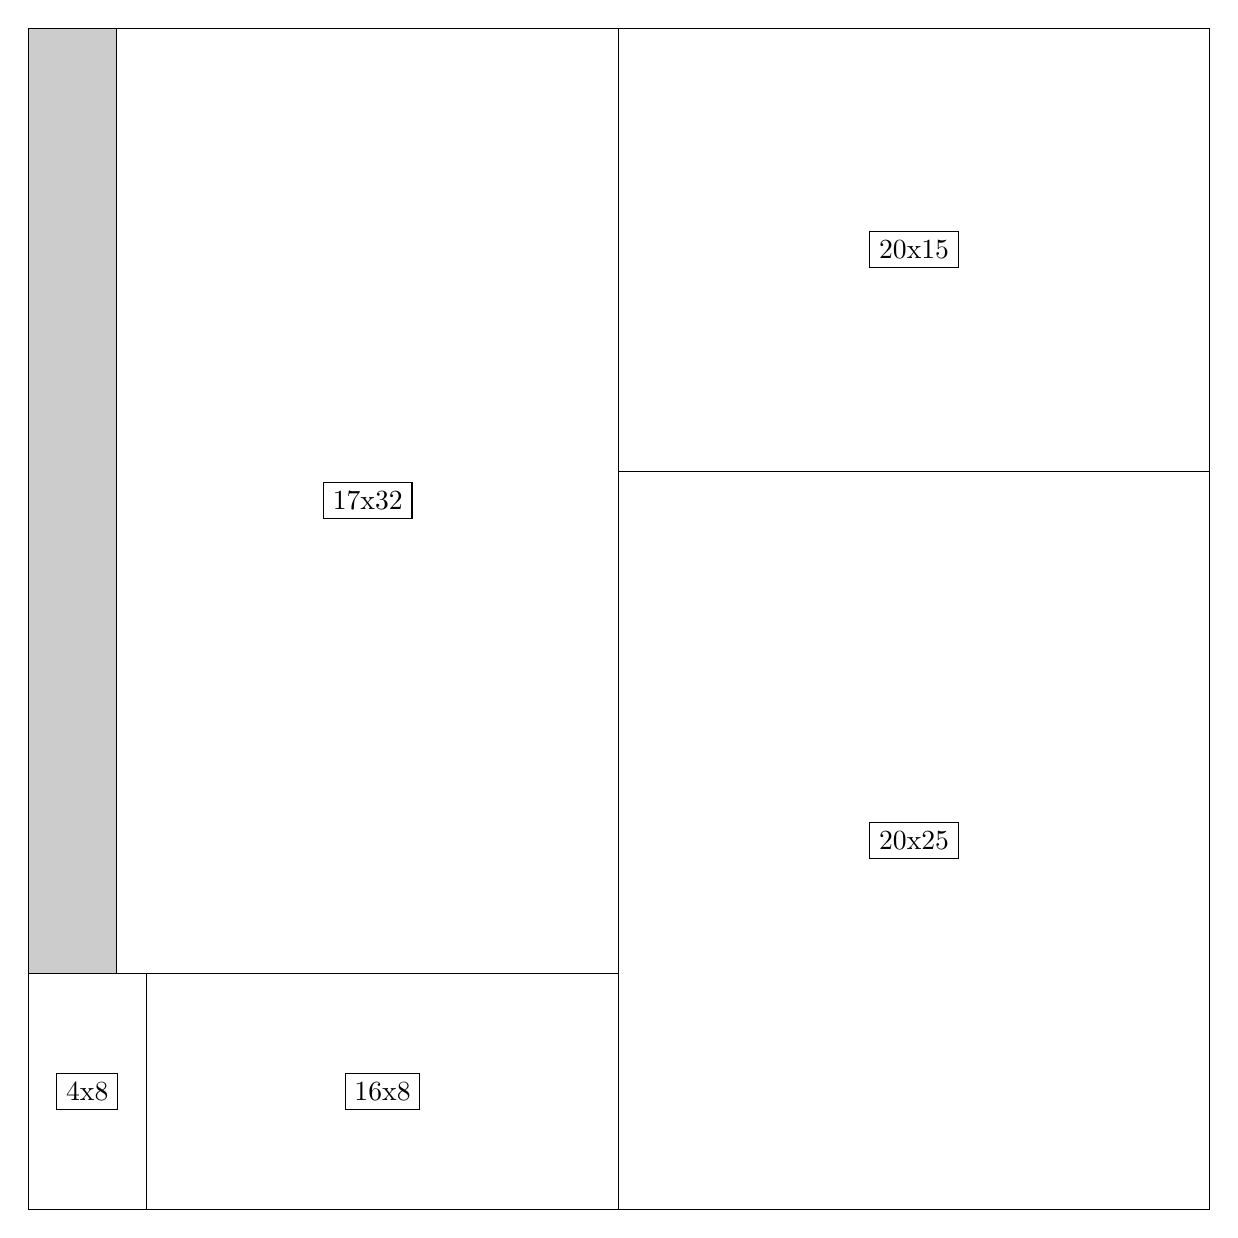
\begin{tikzpicture}[shorten >=1pt,scale=1.0,every node/.style={scale=1.0},->]
\tikzstyle{vertex}=[circle,fill=black!25,minimum size=14pt,inner sep=0pt]
\filldraw[fill=gray!40!white, draw=black] (0,0) rectangle (15.0,15.0);
\foreach \name/\x/\y/\w/\h in {20x25/7.5/0.0/7.5/9.375,20x15/7.5/9.375/7.5/5.625,16x8/1.5/0.0/6.0/3.0,4x8/0.0/0.0/1.5/3.0,17x32/1.125/3.0/6.375/12.0}
\filldraw[fill=white!40!white, draw=black] (\x,\y) rectangle node[draw] (\name) {\name} ++(\w,\h);
\end{tikzpicture}


w =20 , h =25 , x =20 , y =0 , v =500
\par
w =20 , h =15 , x =20 , y =25 , v =300
\par
w =16 , h =8 , x =4 , y =0 , v =128
\par
w =4 , h =8 , x =0 , y =0 , v =32
\par
w =17 , h =32 , x =3 , y =8 , v =544
\par
\newpage


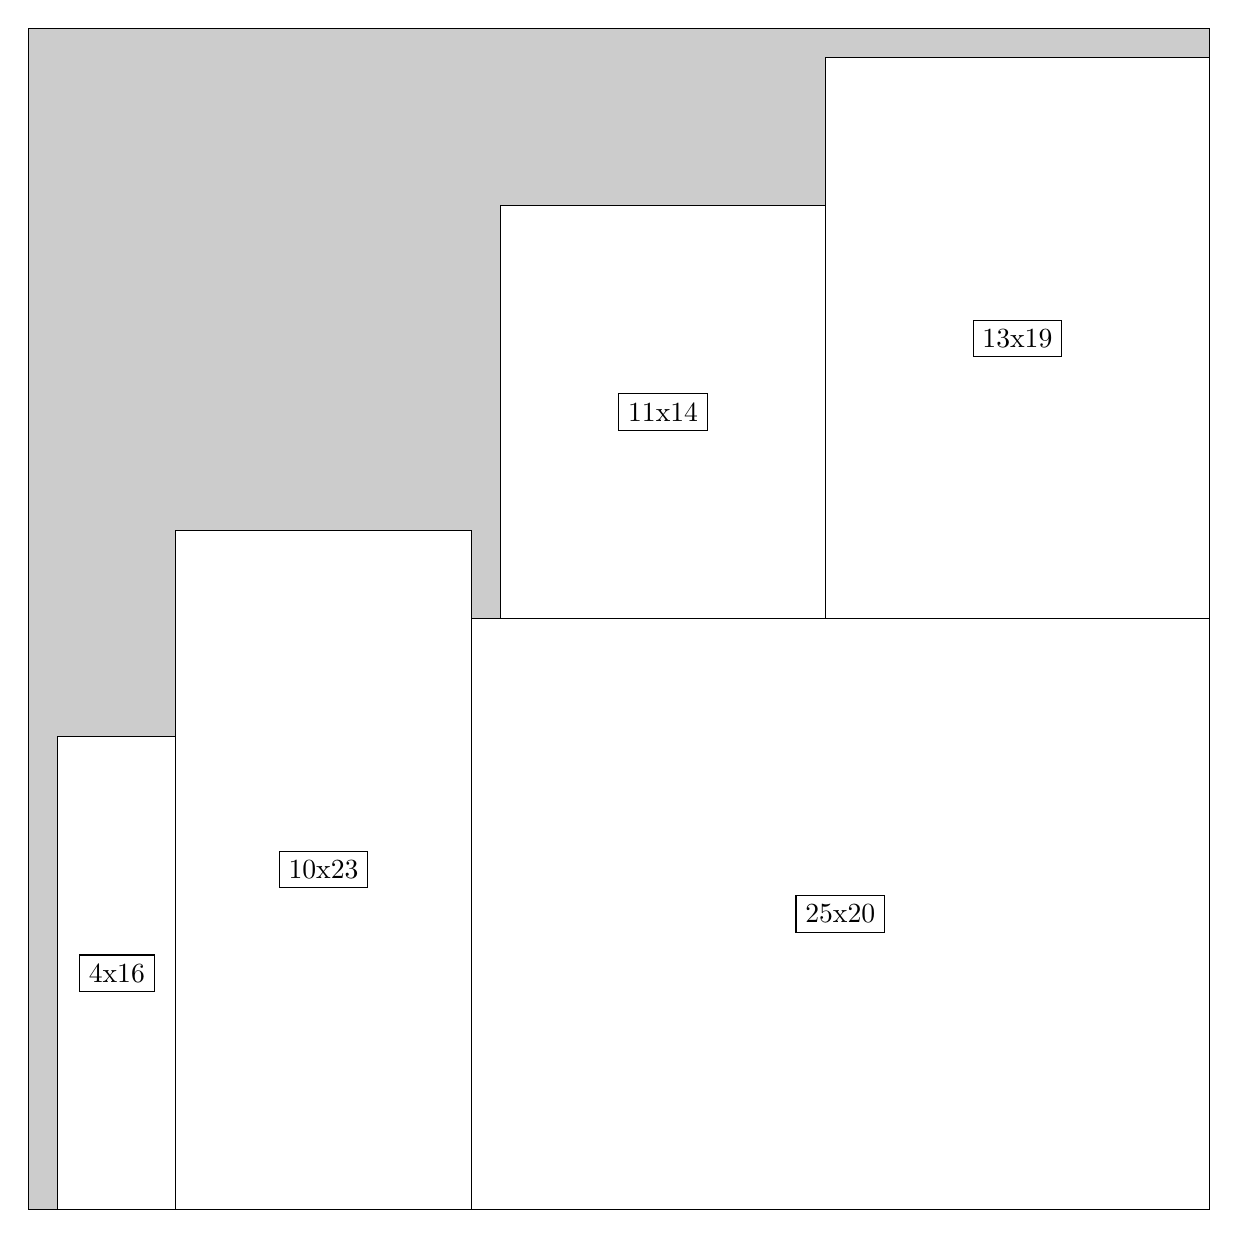
\begin{tikzpicture}[shorten >=1pt,scale=1.0,every node/.style={scale=1.0},->]
\tikzstyle{vertex}=[circle,fill=black!25,minimum size=14pt,inner sep=0pt]
\filldraw[fill=gray!40!white, draw=black] (0,0) rectangle (15.0,15.0);
\foreach \name/\x/\y/\w/\h in {25x20/5.625/0.0/9.375/7.5,13x19/10.125/7.5/4.875/7.125,11x14/6.0/7.5/4.125/5.25,10x23/1.875/0.0/3.75/8.625,4x16/0.375/0.0/1.5/6.0}
\filldraw[fill=white!40!white, draw=black] (\x,\y) rectangle node[draw] (\name) {\name} ++(\w,\h);
\end{tikzpicture}


w =25 , h =20 , x =15 , y =0 , v =500
\par
w =13 , h =19 , x =27 , y =20 , v =247
\par
w =11 , h =14 , x =16 , y =20 , v =154
\par
w =10 , h =23 , x =5 , y =0 , v =230
\par
w =4 , h =16 , x =1 , y =0 , v =64
\par
\newpage


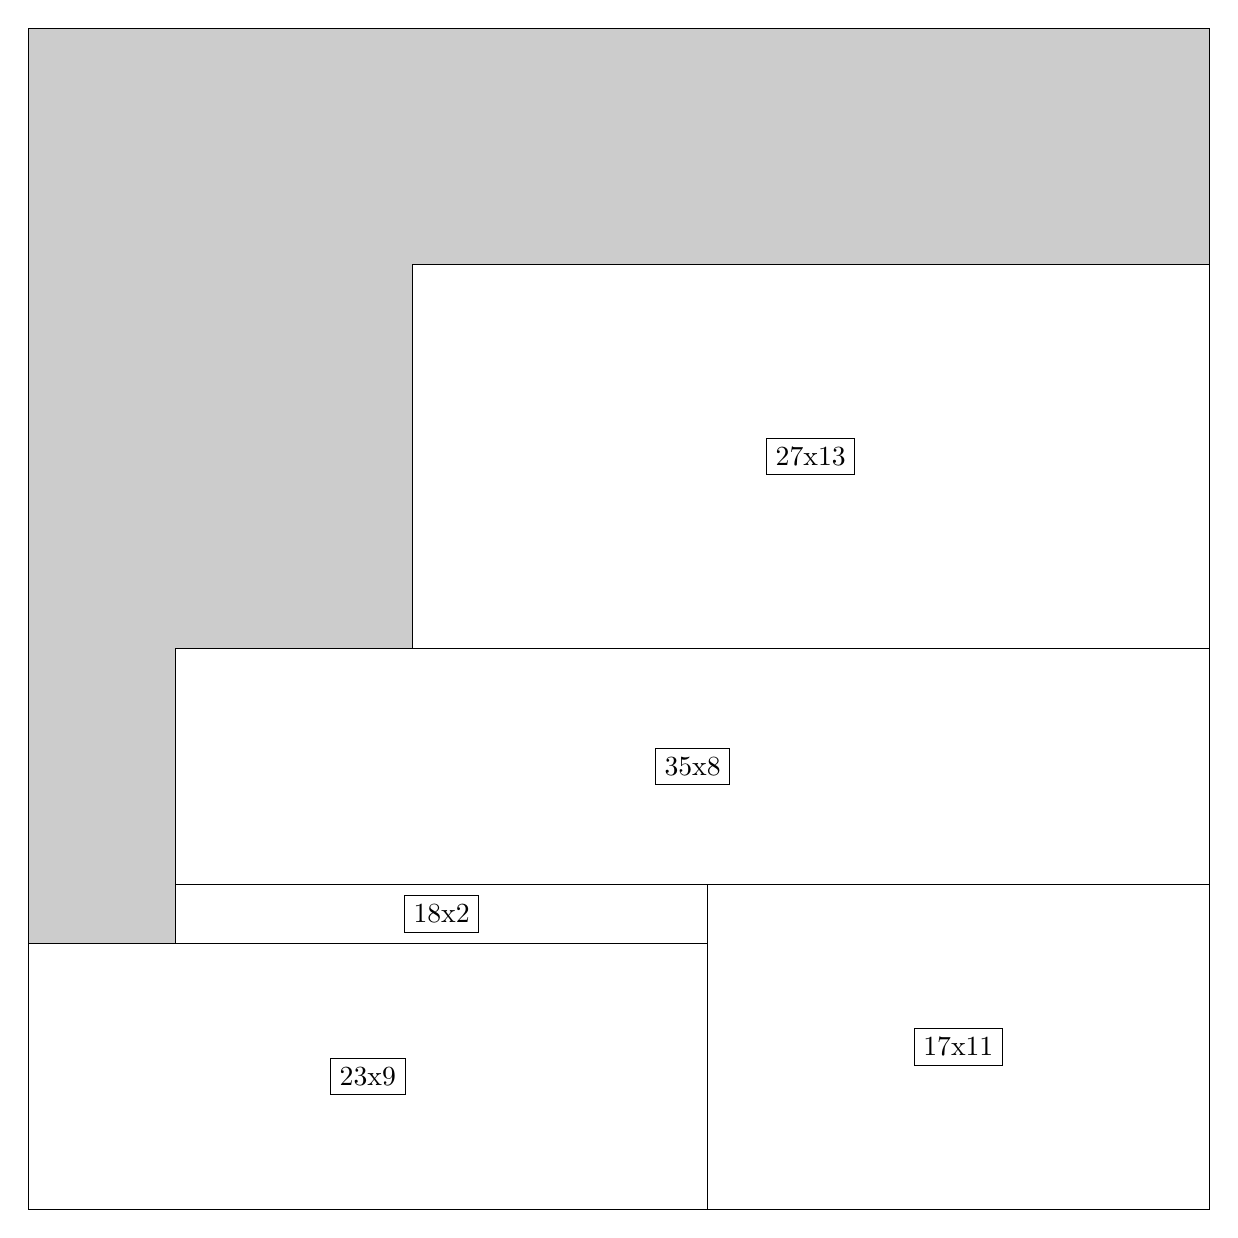
\begin{tikzpicture}[shorten >=1pt,scale=1.0,every node/.style={scale=1.0},->]
\tikzstyle{vertex}=[circle,fill=black!25,minimum size=14pt,inner sep=0pt]
\filldraw[fill=gray!40!white, draw=black] (0,0) rectangle (15.0,15.0);
\foreach \name/\x/\y/\w/\h in {17x11/8.625/0.0/6.375/4.125,23x9/0.0/0.0/8.625/3.375,18x2/1.875/3.375/6.75/0.75,35x8/1.875/4.125/13.125/3.0,27x13/4.875/7.125/10.125/4.875}
\filldraw[fill=white!40!white, draw=black] (\x,\y) rectangle node[draw] (\name) {\name} ++(\w,\h);
\end{tikzpicture}


w =17 , h =11 , x =23 , y =0 , v =187
\par
w =23 , h =9 , x =0 , y =0 , v =207
\par
w =18 , h =2 , x =5 , y =9 , v =36
\par
w =35 , h =8 , x =5 , y =11 , v =280
\par
w =27 , h =13 , x =13 , y =19 , v =351
\par
\newpage


\end{document}